%
% Modo de operación OFB, capítulo de antecedentes.
% Proyecto Lovelace.
%

\subsubsection{\textit{Output Feedback} (OFB)}

Este modo es muy similar al anterior (\acrshort{gl:cfb}), salvo que la
retroalimentación va directamente de la salida del cifrador a bloques. De esta
forma, nada que tenga que ver con el texto en claro llega al cifrado a bloques;
este solamente se la pasa cifrando una y otra vez el
\gls{gl:vector_de_inicializacion}.

\begin{figure}[H]
  \centering
  \begin{subfigure}{0.45\textwidth}
    \begin{center}
      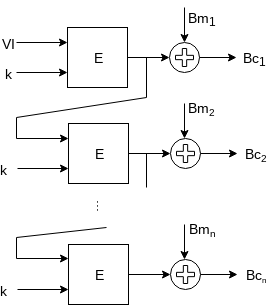
\includegraphics[width=0.7\linewidth]
        {contenidos/antecedentes/bloques/modos/diagramas/modo_ofb.png}
      \caption{Cifrado.}
    \end{center}
  \end{subfigure}
  \begin{subfigure}{0.45\textwidth}
    \begin{center}
      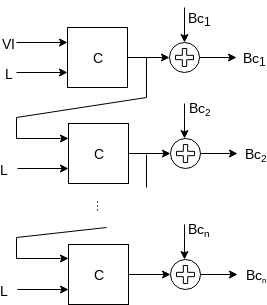
\includegraphics[width=0.7\linewidth]
        {contenidos/antecedentes/bloques/modos/diagramas/modo_ofb_inverso.png}
      \caption{Descifrado.}
    \end{center}
  \end{subfigure}
  \caption{\Gls{gl:modo_de_operacion} \acrshort{gl:ofb}.}
\end{figure}

\begin{pseudocodigo}[%
    caption={\Gls{gl:modo_de_operacion} \acrshort{gl:ofb}%
      (cifrado y descifrado).}%
    ]
  entrada: llave $ L $; vector de inicialización $ VI $;
           bloques de mensaje (cifrado o descifrado) $ B_1, B_2 \dots B_n $.
  salida:  bloques de mensaje (cifrado o descifrado) $ Bc_1, Bc_2 \dots Bc_n $.
  inicio
    auxiliar $\gets$ $ VI $
    para_todo $B$
      auxiliar $\gets$ C($L$, auxiliar)
      $Bc_i$ $\gets$  auxiliar $\oplus$ $B_i$
    fin
    regresar $Bc$
  fin
\end{pseudocodigo}
